\section{Koblitz and binary curves}\label{sec:koblitz}

\subsection{Frobenius-invariant and compact-orbit bases}

The Koblitz implementation (\art{src/cryptanalysis/koblitz_index_calculus.rs})
builds GGMP's invariant base from the linearised polynomial of a factor of
$x^n-1$, checks $\pi(\Fb)=\Fb$ point by point, rewrites each relation into
orbit columns with known $\lambda^k$ weights, and solves the
cofactor-corrected system $h a+hbd\equiv\sum\lambda^{k_i}x_{o_i}$. On
small fields the orbit collapse is as predicted: $\abs\Fb/\#\text{orbits}$
of $7.86$, $10.89$, $12.96$ at $n=9,11,13$ for relations and
$61.7$--$168.0$ for linear algebra, against rho's $4.24$--$5.10$
(\art{RESEARCH_KOBLITZ_INDEX_CALCULUS.md}). Because $\ell=\operatorname{ord}_n(2)$
fixes the invariant base's size, the programme moved to bases sized to the
instance: divisor bases, SAT-optimised bases, a rank-guided base at $n=53$
(220 orbits, a complete implicit $\Sem5$ formula of 22{,}887 clauses), and
finally the \emph{compact signed-Frobenius orbit} base, which stores one
representative per orbit and no pair table
(\art{docs/ic/COMPACT_ORBIT_PRODUCER.md}). In the ecbench factor-base
suite it is the best measured Koblitz construction: $S=9.114$ at $n=17$
($272$ points, 8 columns), $9.985\times$ matched signed-Frobenius rho,
against full orbit $18.7\times$ and subspace bases $47\times$
(\art{research/ecbench_frontier_20261013/}).

\subsection{The oracle sequence}

The binary oracle went through SAT (XOR-native CDCL after Trimoska et
al.~\cite{trimoska2020}; decides the $n=19$, $\ell=6$ corpus but does not
scale), matrix F4 (whose refutation range was the real frontier),
pairs-and-solve for $\Sem4$ (validated to $n=21$, $\ell=7$, still
$O(2^{2\ell})$), meet-in-the-middle pair tables, inherited F4 and F6-IC
(\S\ref{sec:groebner}), and root-finding engines (\S\ref{sec:rootfinding}).
The boundary ledger's current Koblitz decomposition record is an $n=31$,
$m=2$ F4 cell with an exact block-6 M4RI acceleration; at $n=53$ an exact
Frobenius-orbit $\Sem5$ compression removes the coordinate ROM but every
unrestricted solver arm remains \textsc{unknown}.

\subsection{The one-target online ladder}

The ledger's primary \texttt{vs\_rho} question is: with reusable IC
preparation already done, how long does one unseen public target take,
against rho with the automorphism discount on the same point? The ladder
(Figure~\ref{fig:online}):

\begin{itemize}
\item $n=53$: guided shared-log precompute with an explicit pair table
  (9.34\,GB peak RSS); earlier, a 1{,}024-target shared-log batch beat
  batched rho in all 15 paired blocks (secondary, multi-target).
\item $n=61$: compact orbit, 600 columns, 73{,}200 points, 2.73\,GB; fresh
  reproduction $124.85\times$ (exploratory).
\item $n=71$: first rung past 64-bit packing (u128 words), 85{,}200
  points, $2{,}864.1\times$ median of three repeats of one point
  (exploratory).
\item $n=73$: 87{,}600 points, $1{,}189.7\times$; the guided-rank
  precompute took 5.1\,h at 57--70 million probes per relation
  (exploratory).
\item $n=83$, $a=1$: IC online 5.6--7.9\,s against rho 43--71\,s,
  $8.2\times$; then the dense root index, $18.5\times$ (both exploratory).
\item \textbf{$n=61$, admitted} (12 October): $a=0$, $K=500$ orbit
  columns, $61{,}000$ points, 64 fresh public one-target workloads per
  host, identical candidate manifest on two hosts. Pinned x86\_64:
  median online speed-up $13.94\times$, 95\% $[9.81,19.13]$, claim-check
  64/64; unpinned arm64: $12.87\times$ $[7.30,19.08]$. Set-up of about
  28\,s is outside the window; with it charged, IC costs a median
  $83.4\times$ rho.
\end{itemize}

\begin{figure}[t]
\centering
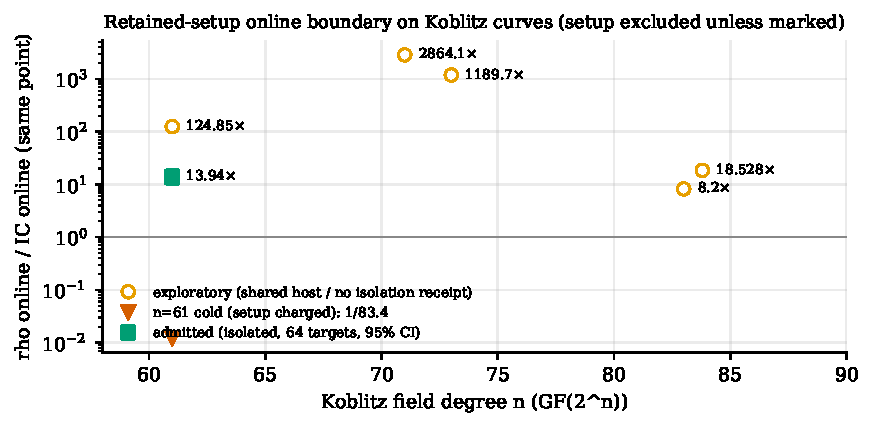
\includegraphics[width=\linewidth]{figures/fig-koblitz-online.pdf}
\caption[]{Rho online time over IC online time on the identical public point,
reusable IC preparation excluded. Open circles: exploratory (verified
answers, no qualifying isolation receipt; three repeats of one point or a
single point). Filled square: the admitted 64-workload panel with its 95\%
bootstrap interval. Triangle: the same $n=61$ candidate with set-up
charged (cold). Sources: \art{docs/ic/boundary_targets.json},
\art{docs/ic/PLAN_IC_ACCOUNTING_FIXES_20261007.md},
\art{research/n83_dense_root_20261013/}.}
\label{fig:online}
\end{figure}

The exploratory ratios are large and irregular because a one-point online
window measures the luck of one relation search against one rho walk; the
admitted panel's range over 64 workloads is $1.06$--$648.6\times$. The
admitted point is a constant-factor online result at $n=61$ (47-bit
subgroup) with preparation retained; it is not a cold result, not a
scaling law, and not an asymptotic claim. By the frontier's own arithmetic
the $n=83$ preparation would pay for itself after $q^*=306$ targets
(derived what-if: reusable set-up $339.0$\,s, online $0.0633$ versus
$1.173$\,s; assumes constant per-target cost and zero rho set-up).

\emph{Retired as an index-calculus win (14 October).} Every rung of this
ladder compares index calculus with a retained table against rho with
none. Given a distinguished-point table of equal or smaller size,
Bernstein--Lange preprocessing rho~\cite{bl2012} is $53$--$317\times$
faster online than the compact-orbit arm on the same 64 targets at $n=41$,
53 and 61 (\S\ref{sec:ladder}). The ladder therefore measures what a
table buys, and generic rho buys more per byte.

\subsection{ECC2K-130}\label{sec:ecc2k130}

ECC2K-130 is the $a=0$, $n=131$ member of the same family; the compact
producer already solves $n=41,53,61,71,73$ of it. Extrapolating the fitted
probes-per-relation law $C\,r/(n^2K^2)$ with $C=1$ gives
$1.1\cdot10^{18}$ core-years at $K=600$ and $6.8\cdot10^{8}$ at
$K=10^{12}$ columns (\art{RESEARCH_ECC2K130_IC_FEASIBILITY.md}, with the
unexplained factor-of-5 gap in $C$ of \S\ref{sec:corrections}). The
separate GPU rho estimate for the same curve is about 4.3 RTX PRO 6000
card-years (\art{paper/ecc2k130/}). Index calculus is not a route to
ECC2K-130 on this evidence; the isogeny-class routes are discussed in
\S\ref{sec:transfer}.
